\chapter{Beeldvorming}
\section{Punten}
\begin{itemize}
	\item Elk 2D punt $(x, y)$ kan gerepresenteerd worden via de \textbf{homogene coördinaten} $(\lambda x, \lambda y, \lambda)$ voor $\lambda \neq 0$. Homogene coördinaten worden ook \textbf{projectieve coördinaten} genoemd, en bevinden zich in het projectieve vlak $\mathcal{P}^2$. 
	\item Het cartesisch punt $(1, 2)$ kan gepresenteerd worden in homogene coördinaten als $(1, 2, 1)$ of zelfs $(2, 4, 2)$.
	\item Het origineel cartesisch punt kan bekomen worden te delen door $\lambda$:
	$$(\lambda x, \lambda y, \lambda) = (\frac{\lambda x}{\lambda}, \frac{\lambda y}{\lambda}, \frac{\lambda}{\lambda}) = (x, y)$$
	\item Een punt kan door oneindig veel homogene coördinaten gerepresenteerd worden.
	\item Dit kan eenvoudig uitgebreid worden in drie dimensies:
	$$(x, y, z, \lambda)$$
\end{itemize}

\section{Lijnen}
\begin{itemize}
	\item Een lineaire vergelijking in $\mathcal{R}^2$ kent een aantal problemen:
	\begin{itemize}
		\item De vergelijking $y = ax + b$ kan geen verticale lijnen voorstellen.
		\item De vergelijking $x = ay + b$ kan geen horizontale lijnen voorstellen.
		\item De vergelijking $ax + by = 1$ kan geen lijnen door de oorsprong voorstellen.
		\item ...
	\end{itemize}
	\item Een lineaire vergelijking in $\mathcal{P}^2$ heeft de volgende vorm:
	$$ax + by + cz = 0$$
	Deze vergelijking kan alle mogelijke lijnstukken voorstellen.
	\item Deze veralgemening lost ook een aantal geometrische problemen op. In $\mathcal{R}^2$ kunnen twee lijnen ofwel elkaar snijden, ofwel nooit snijden. In $\mathcal{P}^2$ snijden twee lijnstukken altijd, maar kan eventueel in oneindig zijn.
\end{itemize}

\section{Twee-dimensionale transformaties}
Figuur \ref{fig:tweedimensionale_transformaties} toont alle transformaties mogelijk in de twee-dimensionale ruimte. 
\begin{figure}[h]
	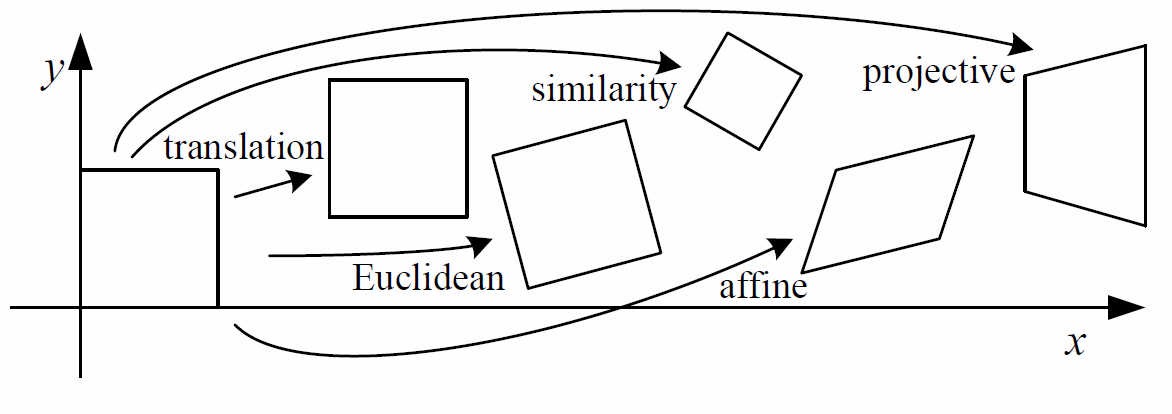
\includegraphics[width=\textwidth]{tweedimensionale_transformaties}
	\caption{Eenvoudige twee-dimensionale transformaties.}
	\label{fig:tweedimensionale_transformaties}
\end{figure}
Elke transformatie maakt gebruik van één of andere matrix. De belangrijkste matrix is die van de projectie:
$$\begin{pmatrix}
x' \\ y' \\ z'
\end{pmatrix}
=
\begin{pmatrix}
h_{11} & h_{12} & h_{13} \\
h_{21} & h_{22} & h_{23} \\
h_{31} & h_{32} & h_{33}
\end{pmatrix}
\begin{pmatrix}
x \\ y \\ z
\end{pmatrix}$$

